\documentclass[../xlapes02]{subfiles}



\begin{document}
    \chapter{Experiments and Results}\label{sec:experiments-and-results}
    In this section we present the results of all the experiments performed. We will also discuss any problems that arose during the conduct of these experiments and provide further information on how we selected certain methods and hyperparameters for more extensive testing.

    By performing a series of experiments, we show how our agent performs in a given environment. We compare the best and worst performing models and discuss the results of our experiments with the baseline models and benchmarks in~\cref{sec:experiments}. We also discuss and compare the hyperparameter settings and the advantages and disadvantages of all the datasets used in~\cref{subsec:hyperparameters}. We also provide some information on how we approached performance testing of the proposed models and what technologies were used for the MLOps concepts, such as tracking training and test runs~\cref{sec:wandb}. Finally, we discuss the results of our experiments and provide a summary of our findings~\cref{sec:summary}.
    \\
    \\
    The computer used for experiments has the following specifications:
    \begin{itemize}
        \item Operating System: Ubuntu 20.04.6 LTS (GNU/Linux 5.4.0-146-generic x86\_64)
        \item CPU: 2 x Intel Xeon CPU E5-2620 v3 @ 2.40GHz, each with six cores, for a total of 12 cores.
        \item RAM: 2 x 32 GB RAM running at 2133MHz, using quad-channel architecture for faster memory access
        \item GPU: 4 x NVIDIA GTX 1080 (Pascal) with 8GB RAM each, providing a total of 32GB GPU memory.
    \end{itemize}
    This configuration is well-suited for AI workloads that can benefit from both CPU and GPU parallelism, such as deep learning. The combination of two Intel Xeon CPUs provides a total of 12 cores, which can be utilized for parallel CPU processing. The 64GB of RAM, along with quad-channel architecture, provides fast access to memory, which is essential for large-scale machine learning tasks. The 4 NVIDIA GTX 1080 GPUs provide additional processing power and GPU memory, which can be leveraged by deep learning frameworks such as TensorFlow or PyTorch to accelerate model training and inference.


    \section{Weights \& Biases}\label{sec:wandb}
    Weights \& Biases (W\&B) is a powerful machine learning experiment tracking and visualization tool that helps data scientists and machine learning practitioners manage their experiments. With W\&B, users can log experiment metrics in real-time, track hyperparameters, and compare and reproduce experiments easily. W\&B offers various visualization tools like interactive plots, histograms, and confusion matrices, which help users analyze and understand experiment results.

    \begin{itemize}
        \item Experiment tracking: W\&B allows users to log experiment metrics such as loss, accuracy, and other custom metrics in real-time during training. These metrics are logged to a central dashboard, making it easy to monitor and compare multiple experiments.
        \item Hyperparameter tuning: W\&B supports hyperparameter sweeps, allowing users to explore different hyperparameter configurations in parallel and find optimal hyperparameter settings for their models.
        \item Visualization: W\&B provides a variety of visualization tools, including interactive graphs, histograms, confusion matrices, and more, to help users analyze and understand experimental results. We use some of the W\&B graphs to compare hyperparameters and their values to understand their effect on the overall range of rewards~\crefrange{fig:wb-chart1}{fig:wb-chart3}.
        \item Artifact management: W\&B allows users to log and version datasets, models, and other artifacts, making it easy to track and reproduce experiments with specific data and model versions.
        \item Collaboration: W\&B enables team collaboration by allowing users to share experiment results, visualizations, and artifacts with team members, facilitating communication and collaboration among team members.
    \end{itemize}

    In this paper, for example, training and test runs are publicly recorded on the W\&B website. The results of each run, including the stored models and datasets, can be found at the following URL: \url{https://wandb.ai/investai/portfolio-allocation}. W\&B provides a rich API that offers many additional features not mentioned in this description. For more information, please refer to the W\&B documentation at \url{https://docs.wandb.ai/} for a detailed description of all features and APIs.


    \section{Experiments}\label{sec:experiments}
    All experiments focused on several metrics. The first is whether the model can outperform standard indices such as the S\&P 500, DJIA and others. Second, what dataset is more appropriate for training the model. The third metric is finding the optimal hyperparameters for the model. And the last metric is the time to train and test the model. All experiments will be described in accordance with our testing period, which is from 2017-01-25 to 2022-12-16.

    \subsection{Hyperparameters}\label{subsec:hyperparameters}
    The hyperparameter sweep was performed on the following hyperparameters with given configuration, and sweep was performed according to the wandb documentation~\cref{sec:wandb}:
    \begin{center}
        \begin{tabular}{|l|c|}
            \hline
            \textbf{Parameter}        & \textbf{Values/range}                           \\ \hline
            policy                    & MlpPolicy                                       \\ \hline
            learning\_rate            & <0.0001, 0.01>                                  \\ \hline
            n\_steps                  & [32, 64, 128, 256, 512, 1024, 2048]             \\ \hline
            gamma                     & <0.9, 0.999>                                    \\ \hline
            gae\_lambda               & <0.8, 0.999>                                    \\ \hline
            ent\_coef                 & <0.0001, 0.01>                                  \\ \hline
            vf\_coef                  & <0.0001, 0.01>                                  \\ \hline
            max\_grad\_norm           & <0.5, 0.99>                                     \\ \hline
            rms\_prop\_eps            & <0.0001, 0.01>                                  \\ \hline
            sde\_sample\_freq         & <4, 32>                                         \\ \hline
            batch\_size               & [32, 64, 128, 256, 512, 1024, 2048, 4096, 8192] \\ \hline
            n\_epochs                 & <1, 10>                                         \\ \hline
            clip\_range               & <0.1, 0.3>                                      \\ \hline
            clip\_range\_vf           & [None, 0.05, 0.1, 0.15, 0.2]                    \\ \hline
            target\_kl                & <0.01, 0.05>                                    \\ \hline
            buffer\_size              & [1000, 2000, 3000, 4000, 5000]                  \\ \hline
            learning\_starts          & <100, 1000>                                     \\ \hline
            tau                       & <0.001, 0.01>                                   \\ \hline
            train\_freq               & <1, 4>                                          \\ \hline
            gradient\_steps           & <1, 4>                                          \\ \hline
            target\_update\_interval  & <1, 4>                                          \\ \hline
            target\_entropy           & <0.1, 0.2>                                      \\ \hline
            policy\_delay             & <1, 4>                                          \\ \hline
            target\_policy\_noise     & <0.1, 0.2>                                      \\ \hline
            target\_noise\_clip       & <0.1, 0.2>                                      \\ \hline
            exploration\_fraction     & <0.1, 0.2>                                      \\ \hline
            exploration\_initial\_eps & <0.1, 0.2>                                      \\ \hline
            exploration\_final\_eps   & <0.1, 0.2>                                      \\ \hline
        \end{tabular}
    \end{center}

    The training was performed with the following algorithms: A2C, PPO, SAC, DDPG, TD3. For each algorithm were hyperparameters chosen randomly from the given range or values. This proces repeats 10 times for each algorithm and dataset. As mentioned earlier, we've used 3 datasets. That means we trained 30 models of each algorithm, with total amount of trained agents 150.

    \begin{figure}
        \centering
        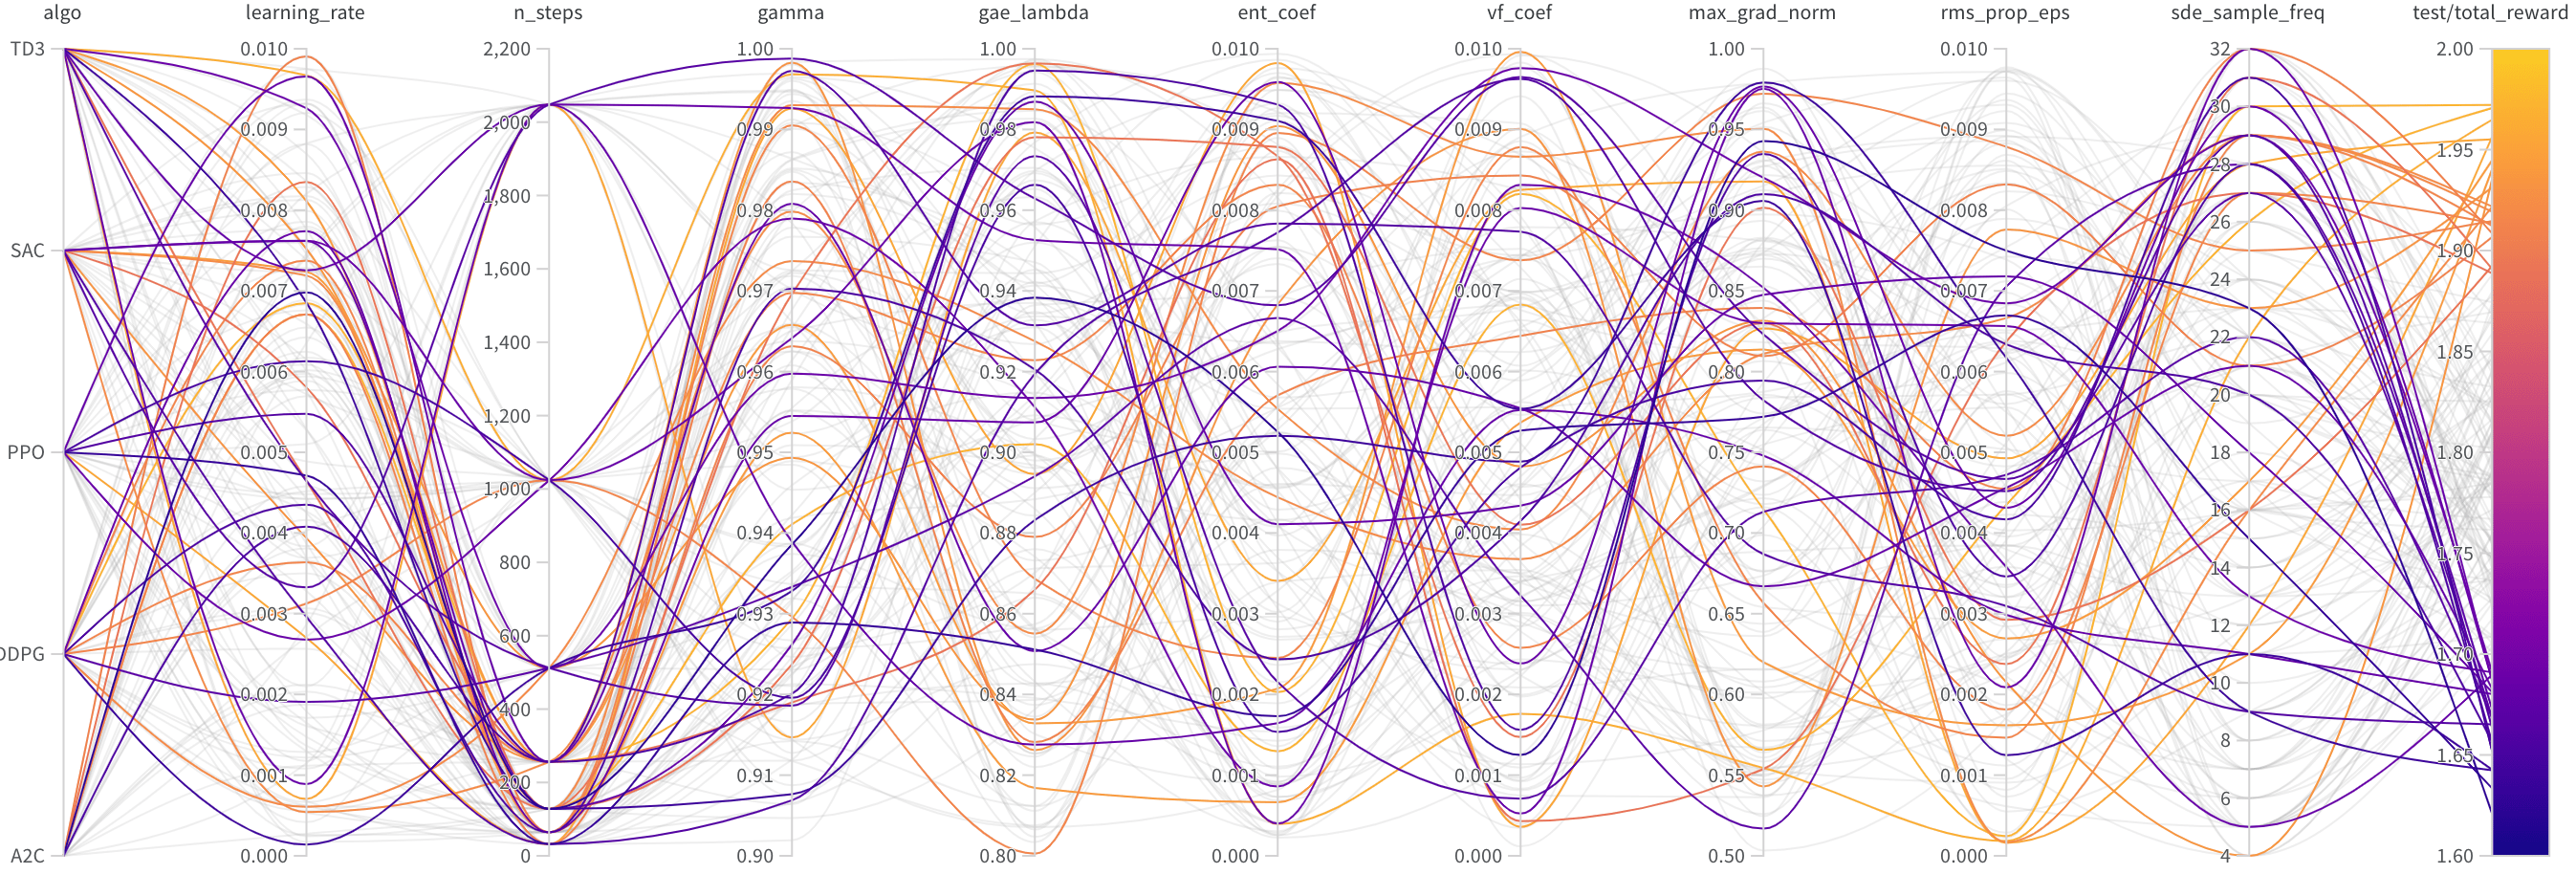
\includegraphics[width=\linewidth, height=0.2\paperheight]{image/figure/wb1}
        \caption{W\&B Chart of parameters and their performance}
        \label{fig:wb-chart1}
    \end{figure}
    \begin{figure}
        \centering
        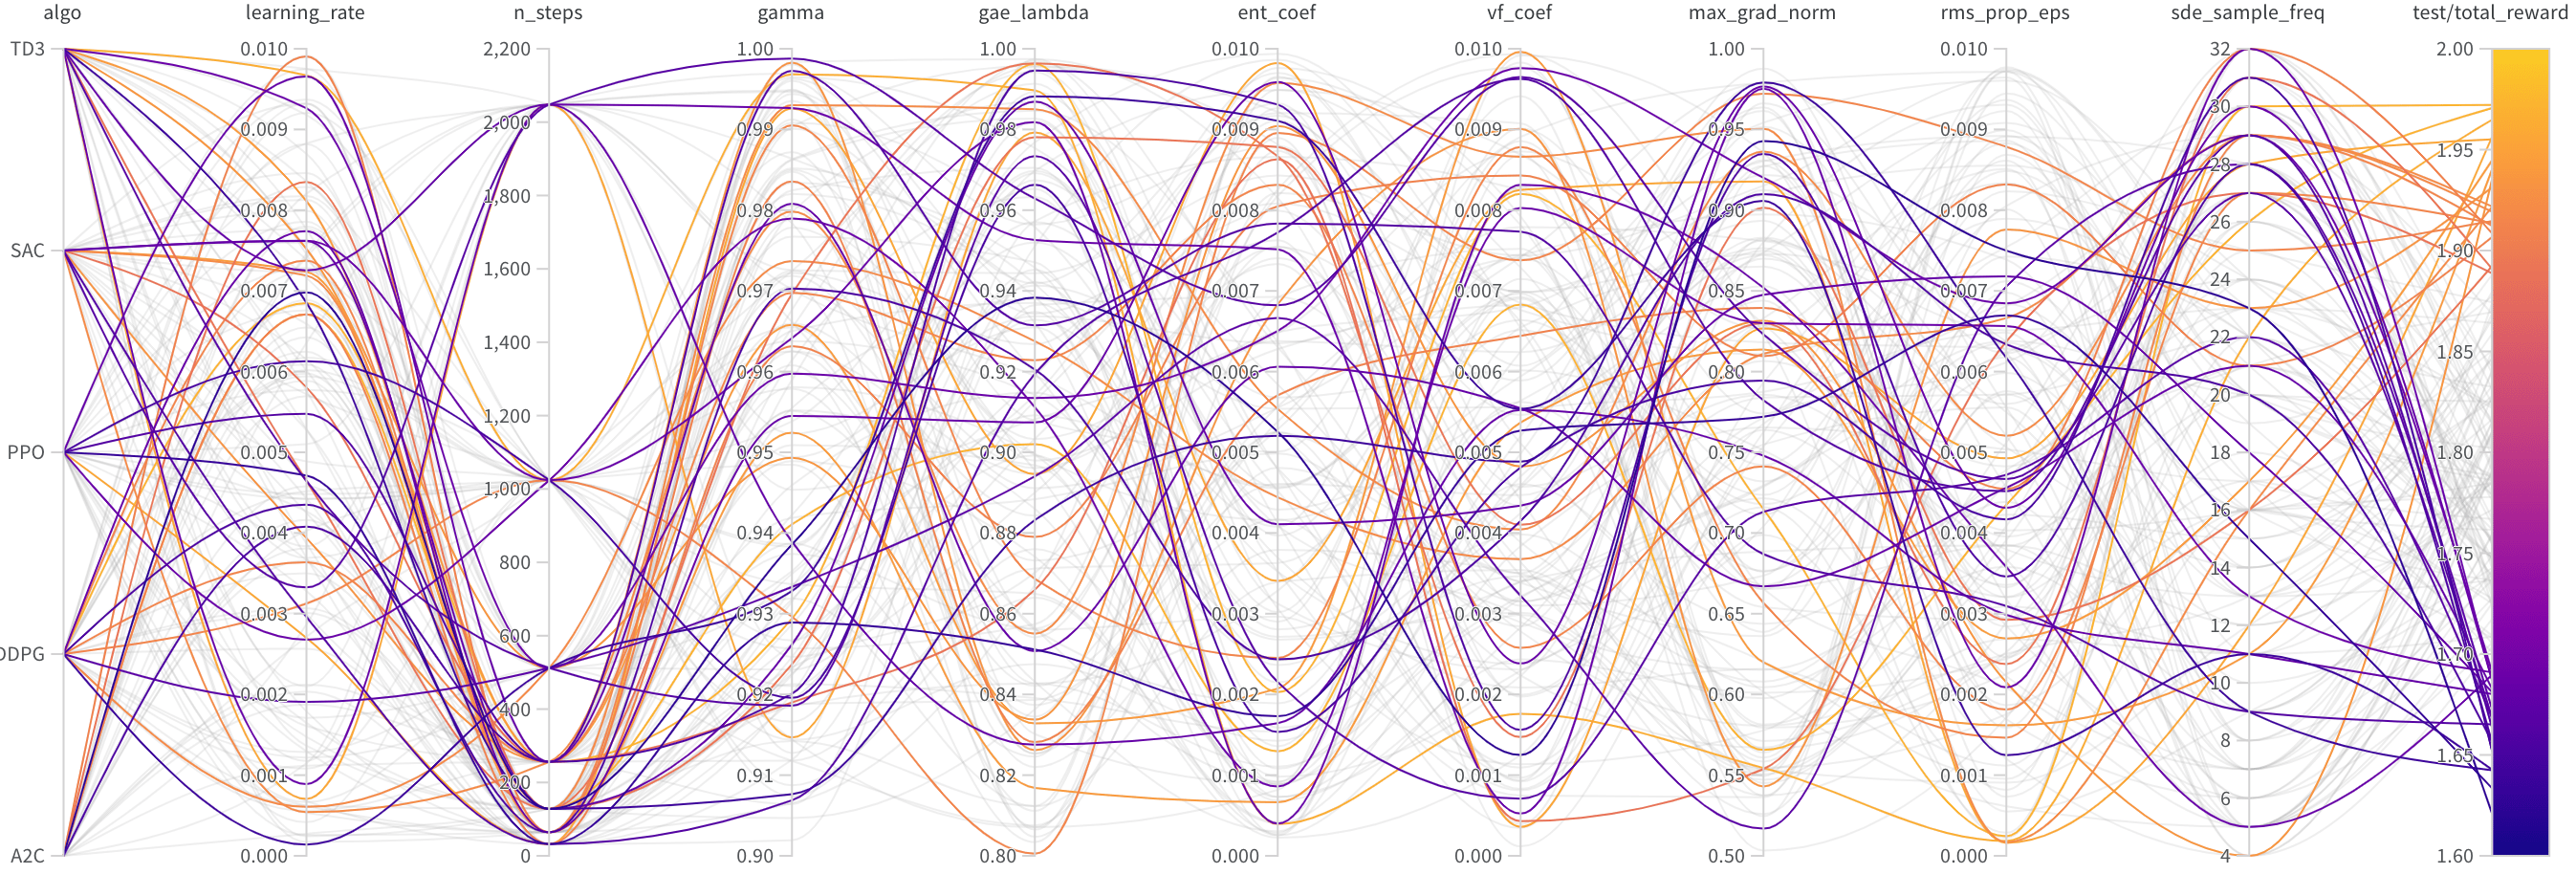
\includegraphics[width=\linewidth, height=0.2\paperheight]{image/figure/wb1}
        \caption{W\&B Chart of parameters and their performance}
        \label{fig:wb-chart2}
    \end{figure}
    \begin{figure}
        \centering
        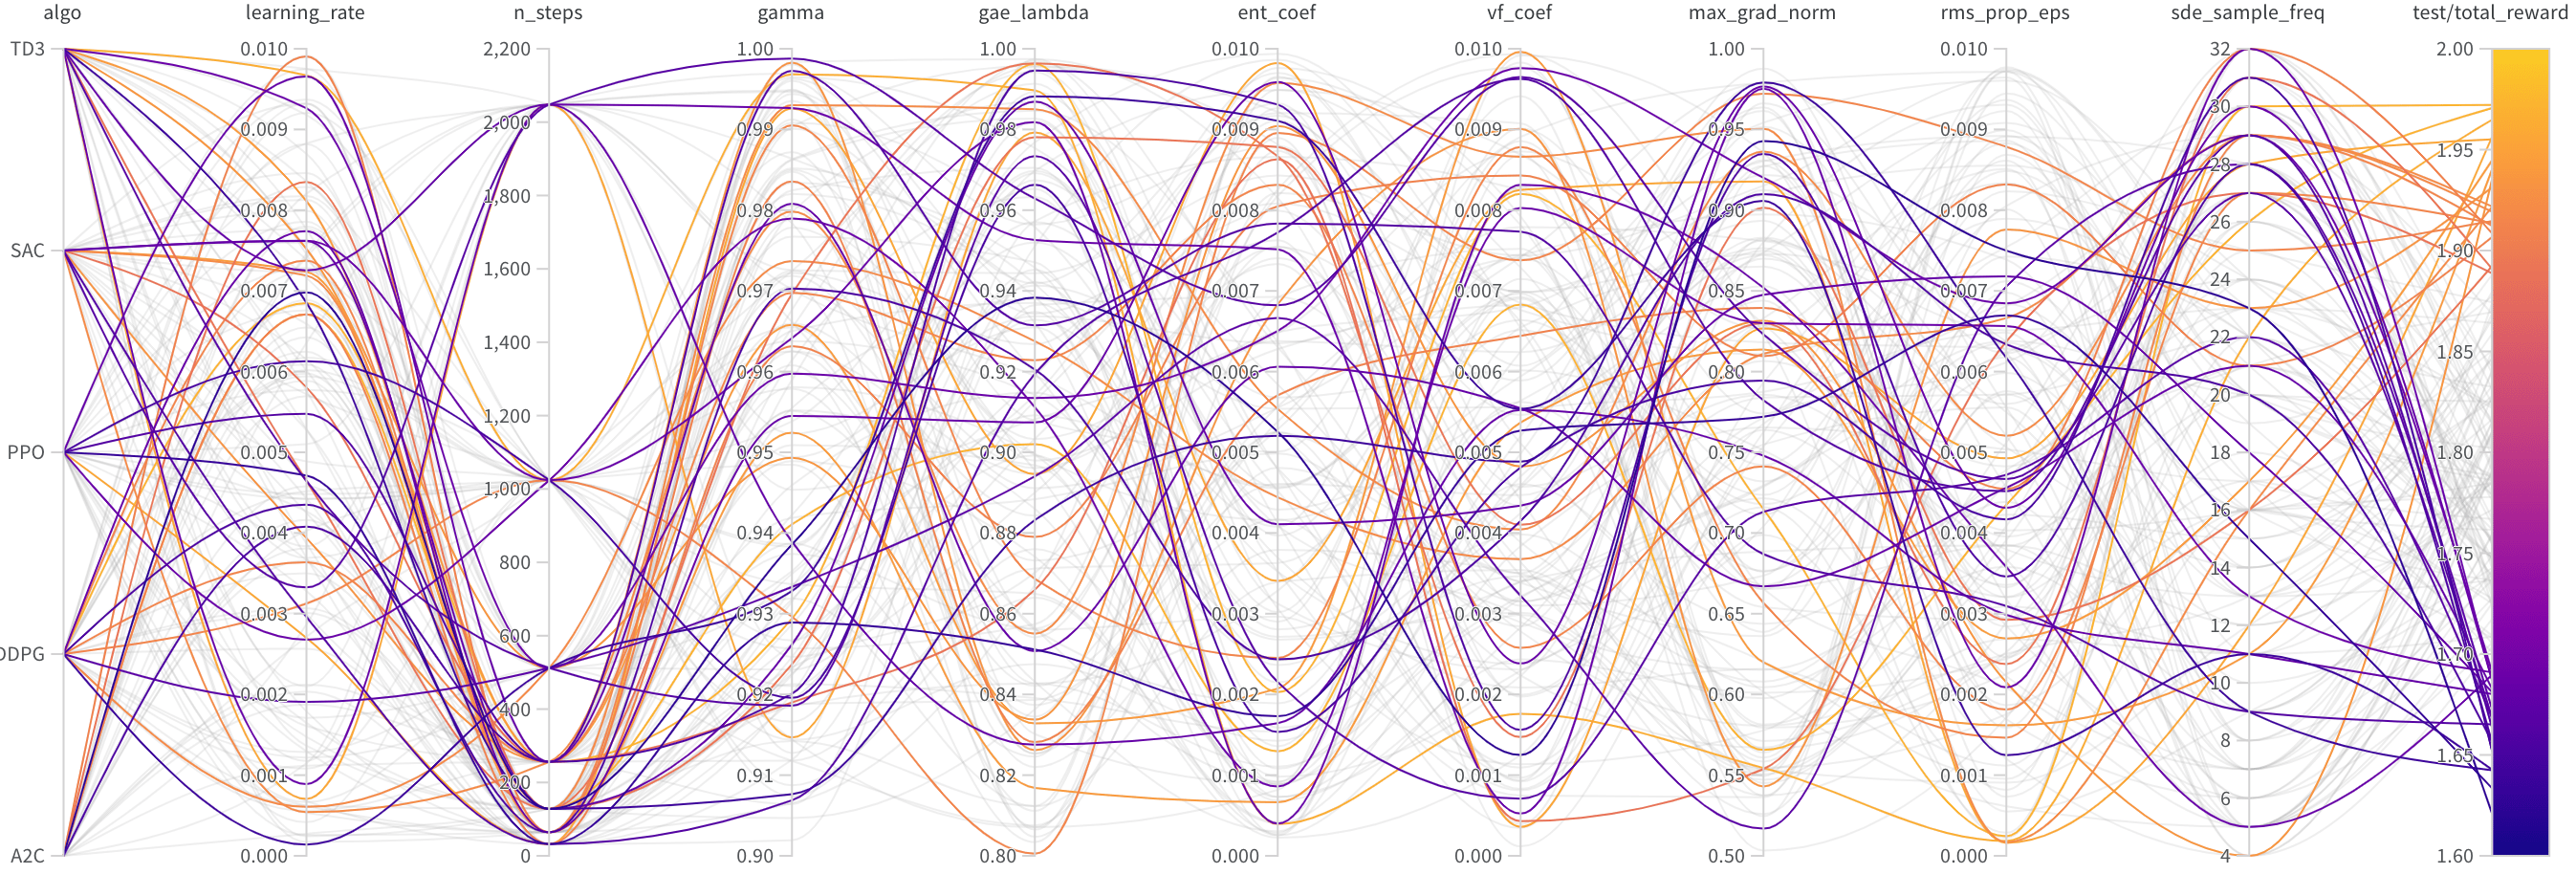
\includegraphics[width=\linewidth, height=0.2\paperheight]{image/figure/wb1}
        \caption{W\&B Chart of parameters and their performance}
        \label{fig:wb-chart3}
    \end{figure}

    We represent the agent performance during the test period in \cref{fig:wb-chart1}. To compare the performance, we chose the \emph{test/total\_reward} attribute, whose value color distinguishes the individual training runs. The higher the reversion (the agent performs better), the color of the curve reaches yellow, while the color changes to purple for poor performance. We can clearly see what parameters are the best for the agent, to achieve the highest performance. The best parameters are:

    \subsection{Baselines and Backtesting}\label{subsec:baselines-and-backtesting}
    In this subsubsection we show, how the agent performs in comparison to the baselines. We use the following baselines:
    \begin{itemize}
        \item \textbf{GSPC} - The S\&P 500 Index is a free-float capitalization-weighted index of the 500 largest publicly traded companies in the United States. The index is maintained by S\&P Dow Jones Indices, a division of S\&P Global. The S\&P 500 index is a price-weighted index, which means that each component stock's price contributes to the index in proportion to its weight. The index is not adjusted for either dividends or splits. It is one of the most commonly followed equity indices.
        \item \textbf{DJI} - The Dow Jones Industrial Average (DJIA), also referred to as the Dow Jones, the Dow 30, or simply the Dow, is a stock market index that measures the stock performance of 30 large companies listed on stock exchanges in the United States. The average is a price-weighted index, which means that each component stock's price contributes to the index in proportion to its weight. The index is not adjusted for either dividends or splits. It is one of the most commonly followed equity indices.
        \item \textbf{RUT} - The Russell 2000 is a stock market index that measures the performance of 2,000 small-cap companies in the United States. It is a subset of the Russell 3000 index, which represents approximately 98\% of the total market capitalization of the US equity market.
        \item \textbf{IXIC} - The NASDAQ Composite is a stock market index that tracks the performance of all the companies listed on the NASDAQ stock exchange, which is primarily composed of technology and growth-oriented companies. The index was launched in 1971 and is considered one of the most widely-followed stock market indices in the world.
        \item \textbf{Minimum Variance} - The Minimum Variance is a portfolio allocation strategy that seeks to minimize the variance of the portfolio's returns. The strategy is based on the assumption that the variance of the portfolio's returns is a measure of risk~\cite{investopedia-portfolio-variance}.
        \item \textbf{Maximum Sharpe Ratio} - The Maximum Sharpe Ratio is a portfolio allocation strategy that seeks to maximize the Sharpe ratio of the portfolio. The strategy is based on the assumption that the Sharpe ratio is a measure of risk-adjusted return~\cite{investopedia-sharpe-ratio}.
    \end{itemize}

    \begin{figure}[h!]
        \centering
        \begin{subfigure}[t]{\experimentimgwidth\textwidth}
            \centering
            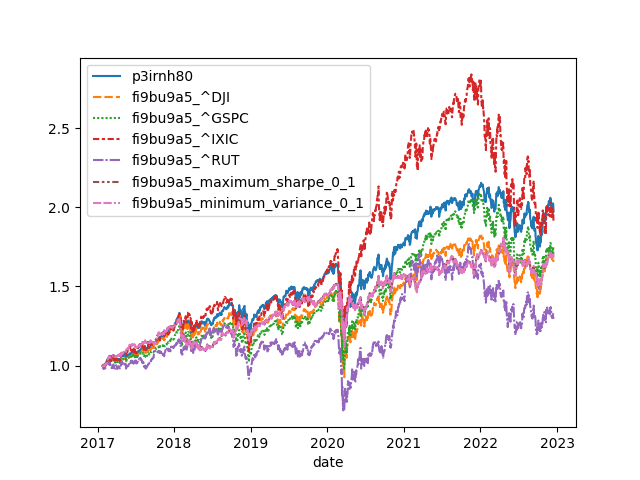
\includegraphics[width=\linewidth]{image/figure/returns_max}
            \caption{The model with The Highest Cumulative Reward}
            \label{fig:returns_max}
        \end{subfigure}
        \hfill
        \begin{subfigure}[t]{\experimentimgwidth\textwidth}
            \centering
            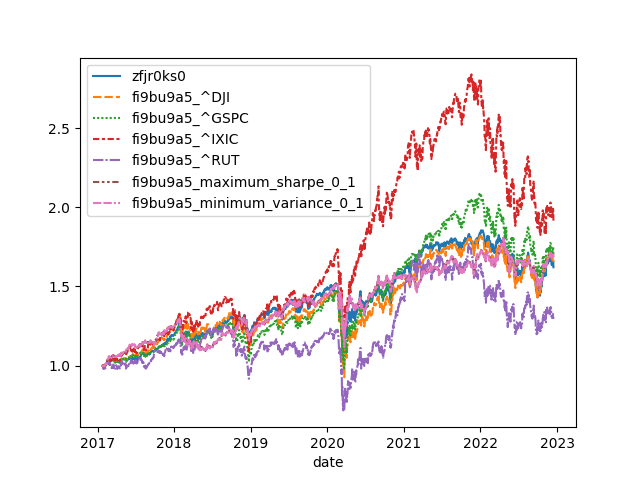
\includegraphics[width=\linewidth]{image/figure/returns_min}
            \caption{The model with The Smallest Cumulative Reward}
            \label{fig:returns_min}
        \end{subfigure}
        \vspace{0.5cm}
        \begin{subfigure}[t]{\experimentimgwidth\textwidth}
            \centering
            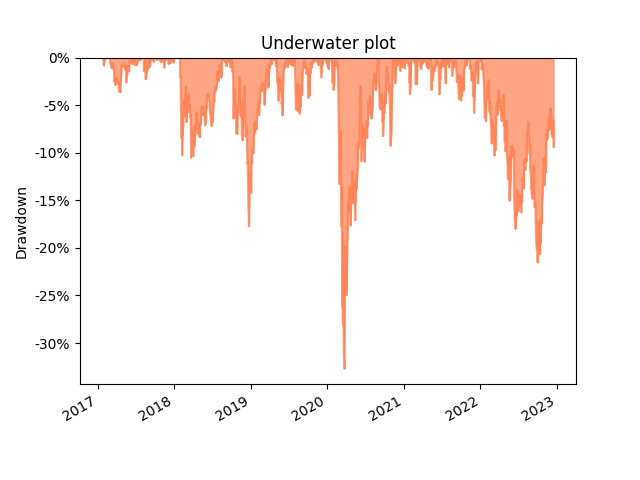
\includegraphics[width=\linewidth]{image/figure/drawdown_underwater_max}
            \caption{The model with The Highest Cumulative Reward}
            \label{fig:drawdown_underwater_max}
        \end{subfigure}
        \hfill
        \begin{subfigure}[t]{\experimentimgwidth\textwidth}
            \centering
            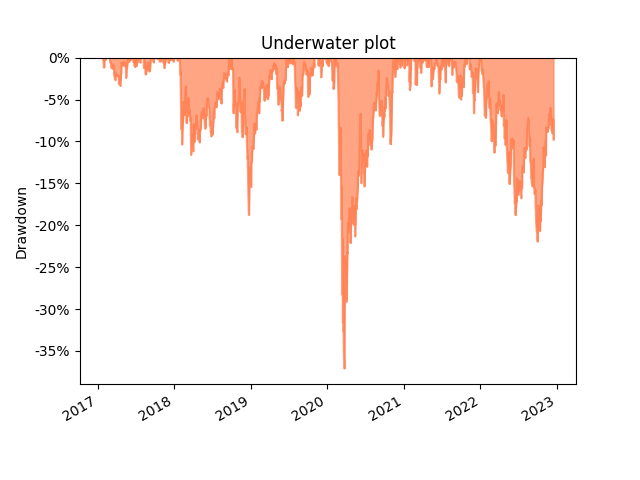
\includegraphics[width=\linewidth]{image/figure/drawdown_underwater_dji}
            \caption{The DJI index}
            \label{fig:drawdown_underwater_dji}
        \end{subfigure}
        \caption{Cumulative return.}
        \label{fig:cumulative_return}
    \end{figure}

    The image~\cref{fig:cumulative_return} illustrates that a model can produce good results if it is configured with appropriate hyperparameters. Conversely, a model that is not configured with suitable hyperparameters fails to generate satisfactory results. The model that performs the best with optimal hyperparameters surpasses standard indexes such as S\&P 500 and DJIA, whereas the model that performs the worst with inadequate hyperparameters cannot outperform these benchmarks. How we tune hyperparameters is described in~\cref{subsec:hyperparameters}

    If we look at the draw-down graphs in~\cref{fig:cumulative_return}, we can see that our tuned model is much better than DJI index at large drawdowns, even both our models perform very well compared to the DJI index.


    \begin{figure}[h!]
        \centering
        %
        \begin{subfigure}[t]{\experimentimgwidth\textwidth}
            \centering
            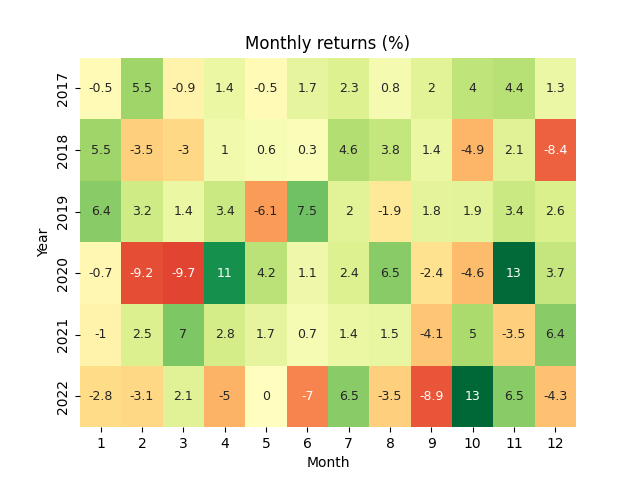
\includegraphics[width=\linewidth]{image/figure/monthly_returns_heatmap_max}
            \caption{The model with the highest cumulative reward}
        \end{subfigure}
        \hfill
        \begin{subfigure}[t]{\experimentimgwidth\textwidth}
            \centering
            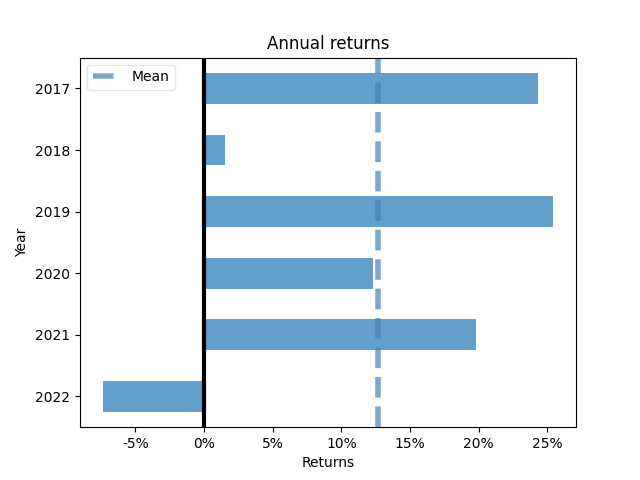
\includegraphics[width=\linewidth]{image/figure/annual_returns_max}
            \caption{The model with the highest cumulative reward}
        \end{subfigure}
        \vspace{0.5cm}

        %
        \begin{subfigure}[t]{\experimentimgwidth\textwidth}
            \centering
            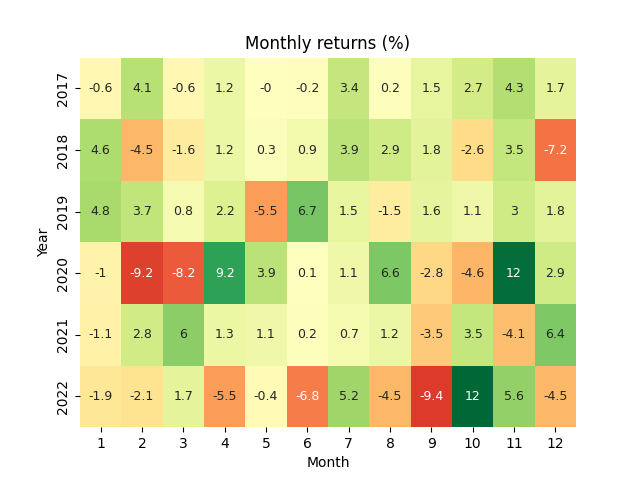
\includegraphics[width=\linewidth]{image/figure/monthly_returns_heatmap_min}
            \caption{The model with the smallest cumulative reward}
        \end{subfigure}
        \hfill
        \begin{subfigure}[t]{\experimentimgwidth\textwidth}
            \centering
            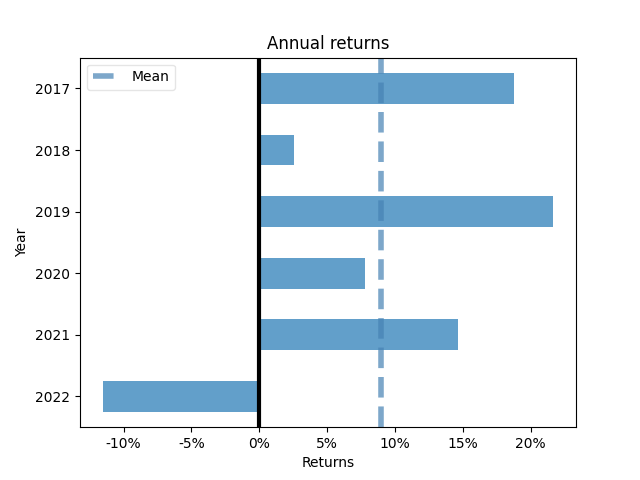
\includegraphics[width=\linewidth]{image/figure/annual_returns_min}
            \caption{The model with the smallest cumulative reward}
        \end{subfigure}
        \vspace{0.5cm}

        %
        \begin{subfigure}[t]{\experimentimgwidth\textwidth}
            \centering
            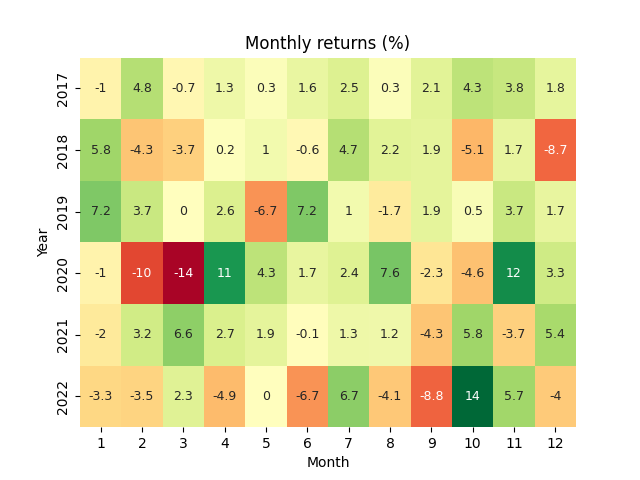
\includegraphics[width=\linewidth]{image/figure/monthly_returns_heatmap_dji}
            \caption{The DJI index}
        \end{subfigure}
        \hfill
        \begin{subfigure}[t]{\experimentimgwidth\textwidth}
            \centering
            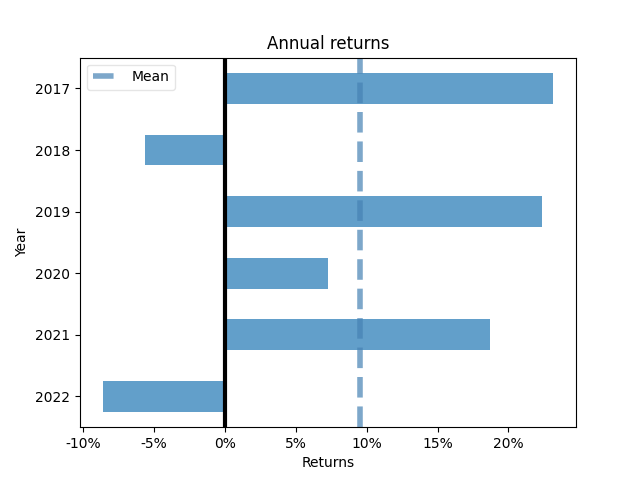
\includegraphics[width=\linewidth]{image/figure/annual_returns_dji}
            \caption{The DJI index}
        \end{subfigure}

        %
        \caption{The monthly returns.}
        \label{fig:month_annual_returns}
    \end{figure}

    % TODO: tabel with best models hyperparameters and dataset name


    \section{Summary}\label{sec:summary}
    TODO


\end{document}
